\selectlanguage{english}%

\section{Approach}


\subsection{The Data}

The data is not given as a classic table and therefor not directly
useable for classification. It consists of two sets of images. The
first one contains the original images of each cross section and a
corresponding mask. A mask is a grayscale image with only black or
white pixels. A pixel is white if it belongs to the cross section
and black if it does not. There are $762$ images with a resolution
of $3272\times2469$, resulting in a huge amount of pixels.

\begin{lstlisting}[caption=libsvm format,label=lisbsvm] 
<class_label> <feature_id>:value ... <feature_id>:value
<class_label> <feature_id>:value ... <feature_id>:value ... 
\end{lstlisting} 

The classification problem is a binary one since there are only two
classes. Before a classifier can be trained, the images have to be
converted into a attribute value format. The libsvm format was chosen,
because it is well known and many libraries support it. Every row
represents one instance, which is in this case one pixel and its features.
Currently the only features available are the rgb values of a pixel
from the original image and the class label from the mask. 


\subsection{Data Preparation}

In the first preprocessing step the libsvm data is created. The easiest
method saves for each pixel the rgb values and the class label. This
is done for every image resulting in $762$ files. Every file has
$8.078.568$ instances, so there are $6.155.868.816$ pixels in total.
A first trivial approach took about 3 days to generate all attribute
value files.

Building a model on this set would take a huge amount of time and
is therefor unreasonable for selecting a model. Instead of using the
complete data set samples have to be used. As figure \ref{fig:mask603}
shows there are more instances of class $0$ (black pixels) than of
class $1$ (white pixels). To weight both classes equally, the sampled
set is balanced. 

\begin{figure}	
\centering 	
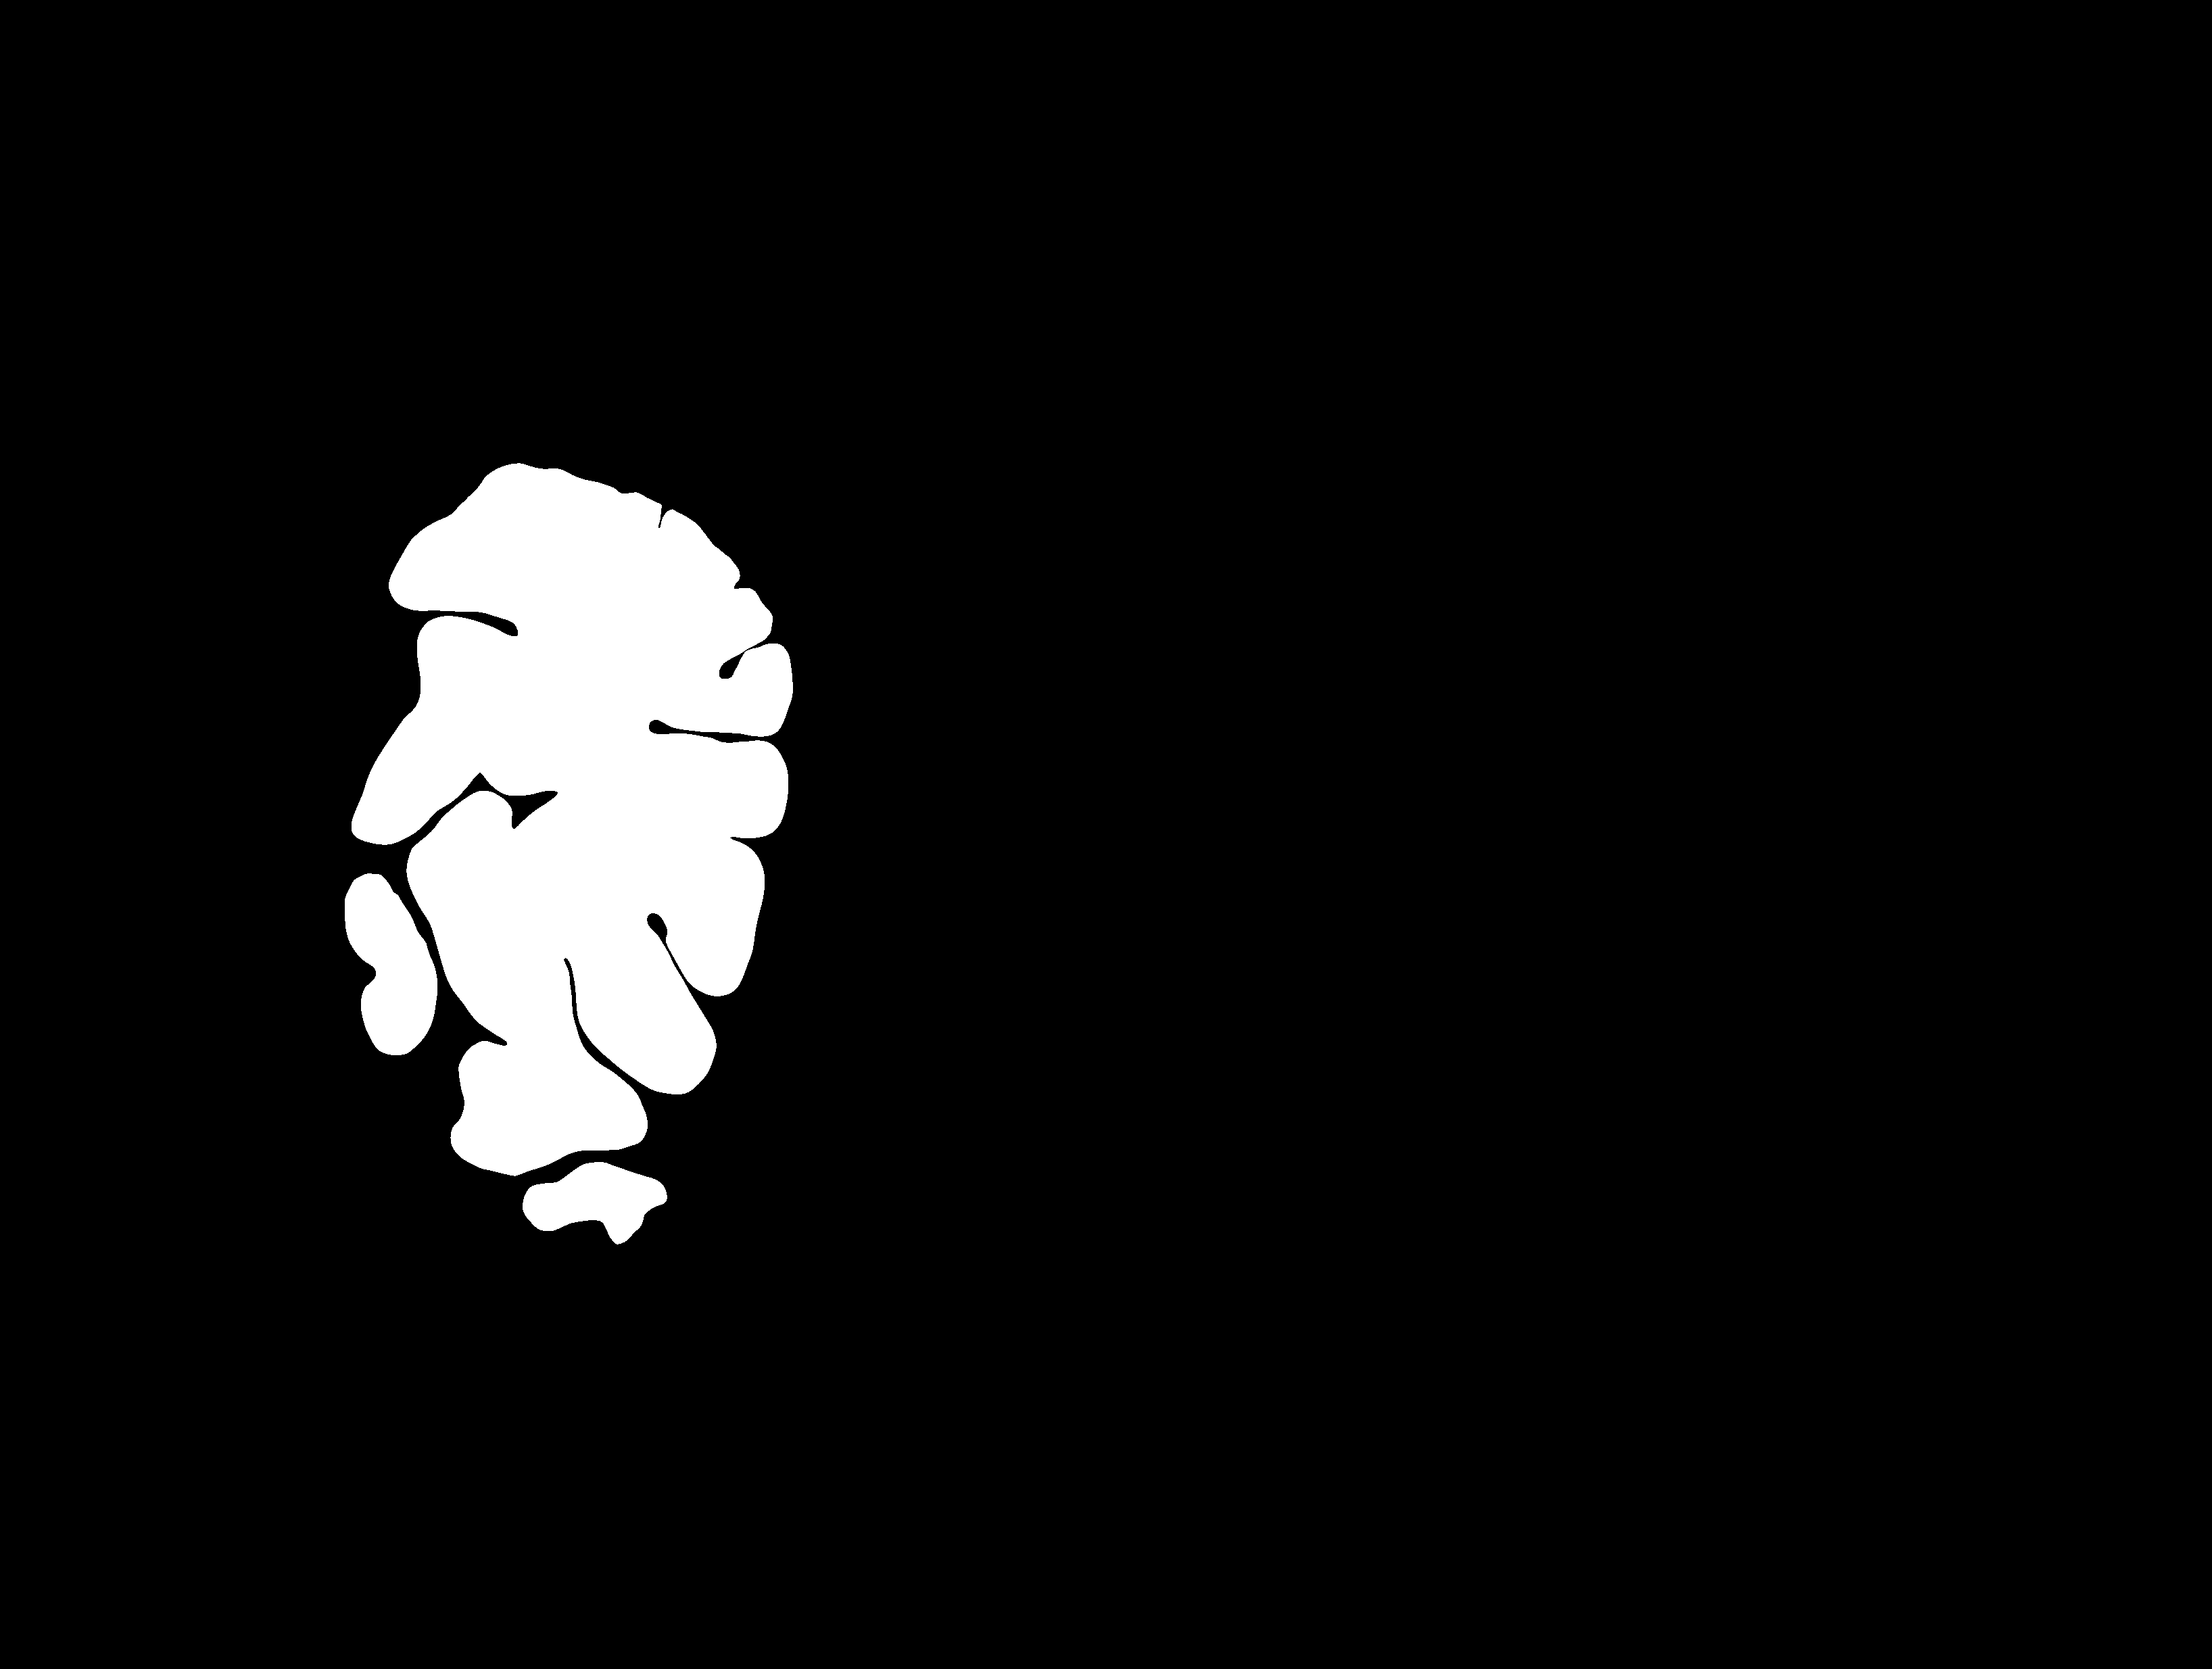
\includegraphics[width=0.6\linewidth]{graphics/mask200} 	
\caption{Mask of a cross section} 	
\label{fig:mask603} 
\end{figure}

The first approach is a balanced random sampling method. For a given
percentage $p$ and a data set with $N$ instances the method draws
$p\cdot N$ samples from a file. If the sample is balanced, $p\cdot N\cdot0.5$
instances of each class are drawn randomly. This can easily be parallelized
since the files can be sampled independently. This yields a first
sample with three features. To improve the classifier the number of
features has to be increased.


\subsubsection{HSV color space}

An easy method to increase the number of features is to use another
color space in addition to the given RGB values. In this case the
HSV color space was chosen. It represents a color by its hue, saturation
and value. The values for a pixel can easily be transformed from RGB
to HSV with the following formula:

\begin{eqnarray*}
Max & = & max(R,G,B)\\
Min & = & min(R,G,B)\\
H & = & \begin{cases}
0, & \text{if Max =Min \ensuremath{\Leftrightarrow}}R=G=B\\
60\text{\textdegree}\cdot\left(0+\frac{G-B}{Max-Min}\right) & \text{if Max =R }\\
60\text{\textdegree}\cdot\left(2+\frac{B-R}{Max-Min}\right) & \text{if Max =G}\\
60\text{\textdegree}\cdot\left(4+\frac{R-G}{Max-Min}\right) & \text{if Max =B}
\end{cases}\\
S & = & \begin{cases}
0 & \text{if Max =0 \ensuremath{\Leftrightarrow}R=G=B=0 }\\
\frac{Max-Min}{Max} & else
\end{cases}\\
V & = & Max
\end{eqnarray*}


Since this computation can be done independently for every pixel,
the features can easily be computed in parallel and be added to existing
data. While computing the HSV values is simple, they also add only
few additional information. Because of this the increase of accuracy
is only marginal.

\begin{figure} 
\centering 
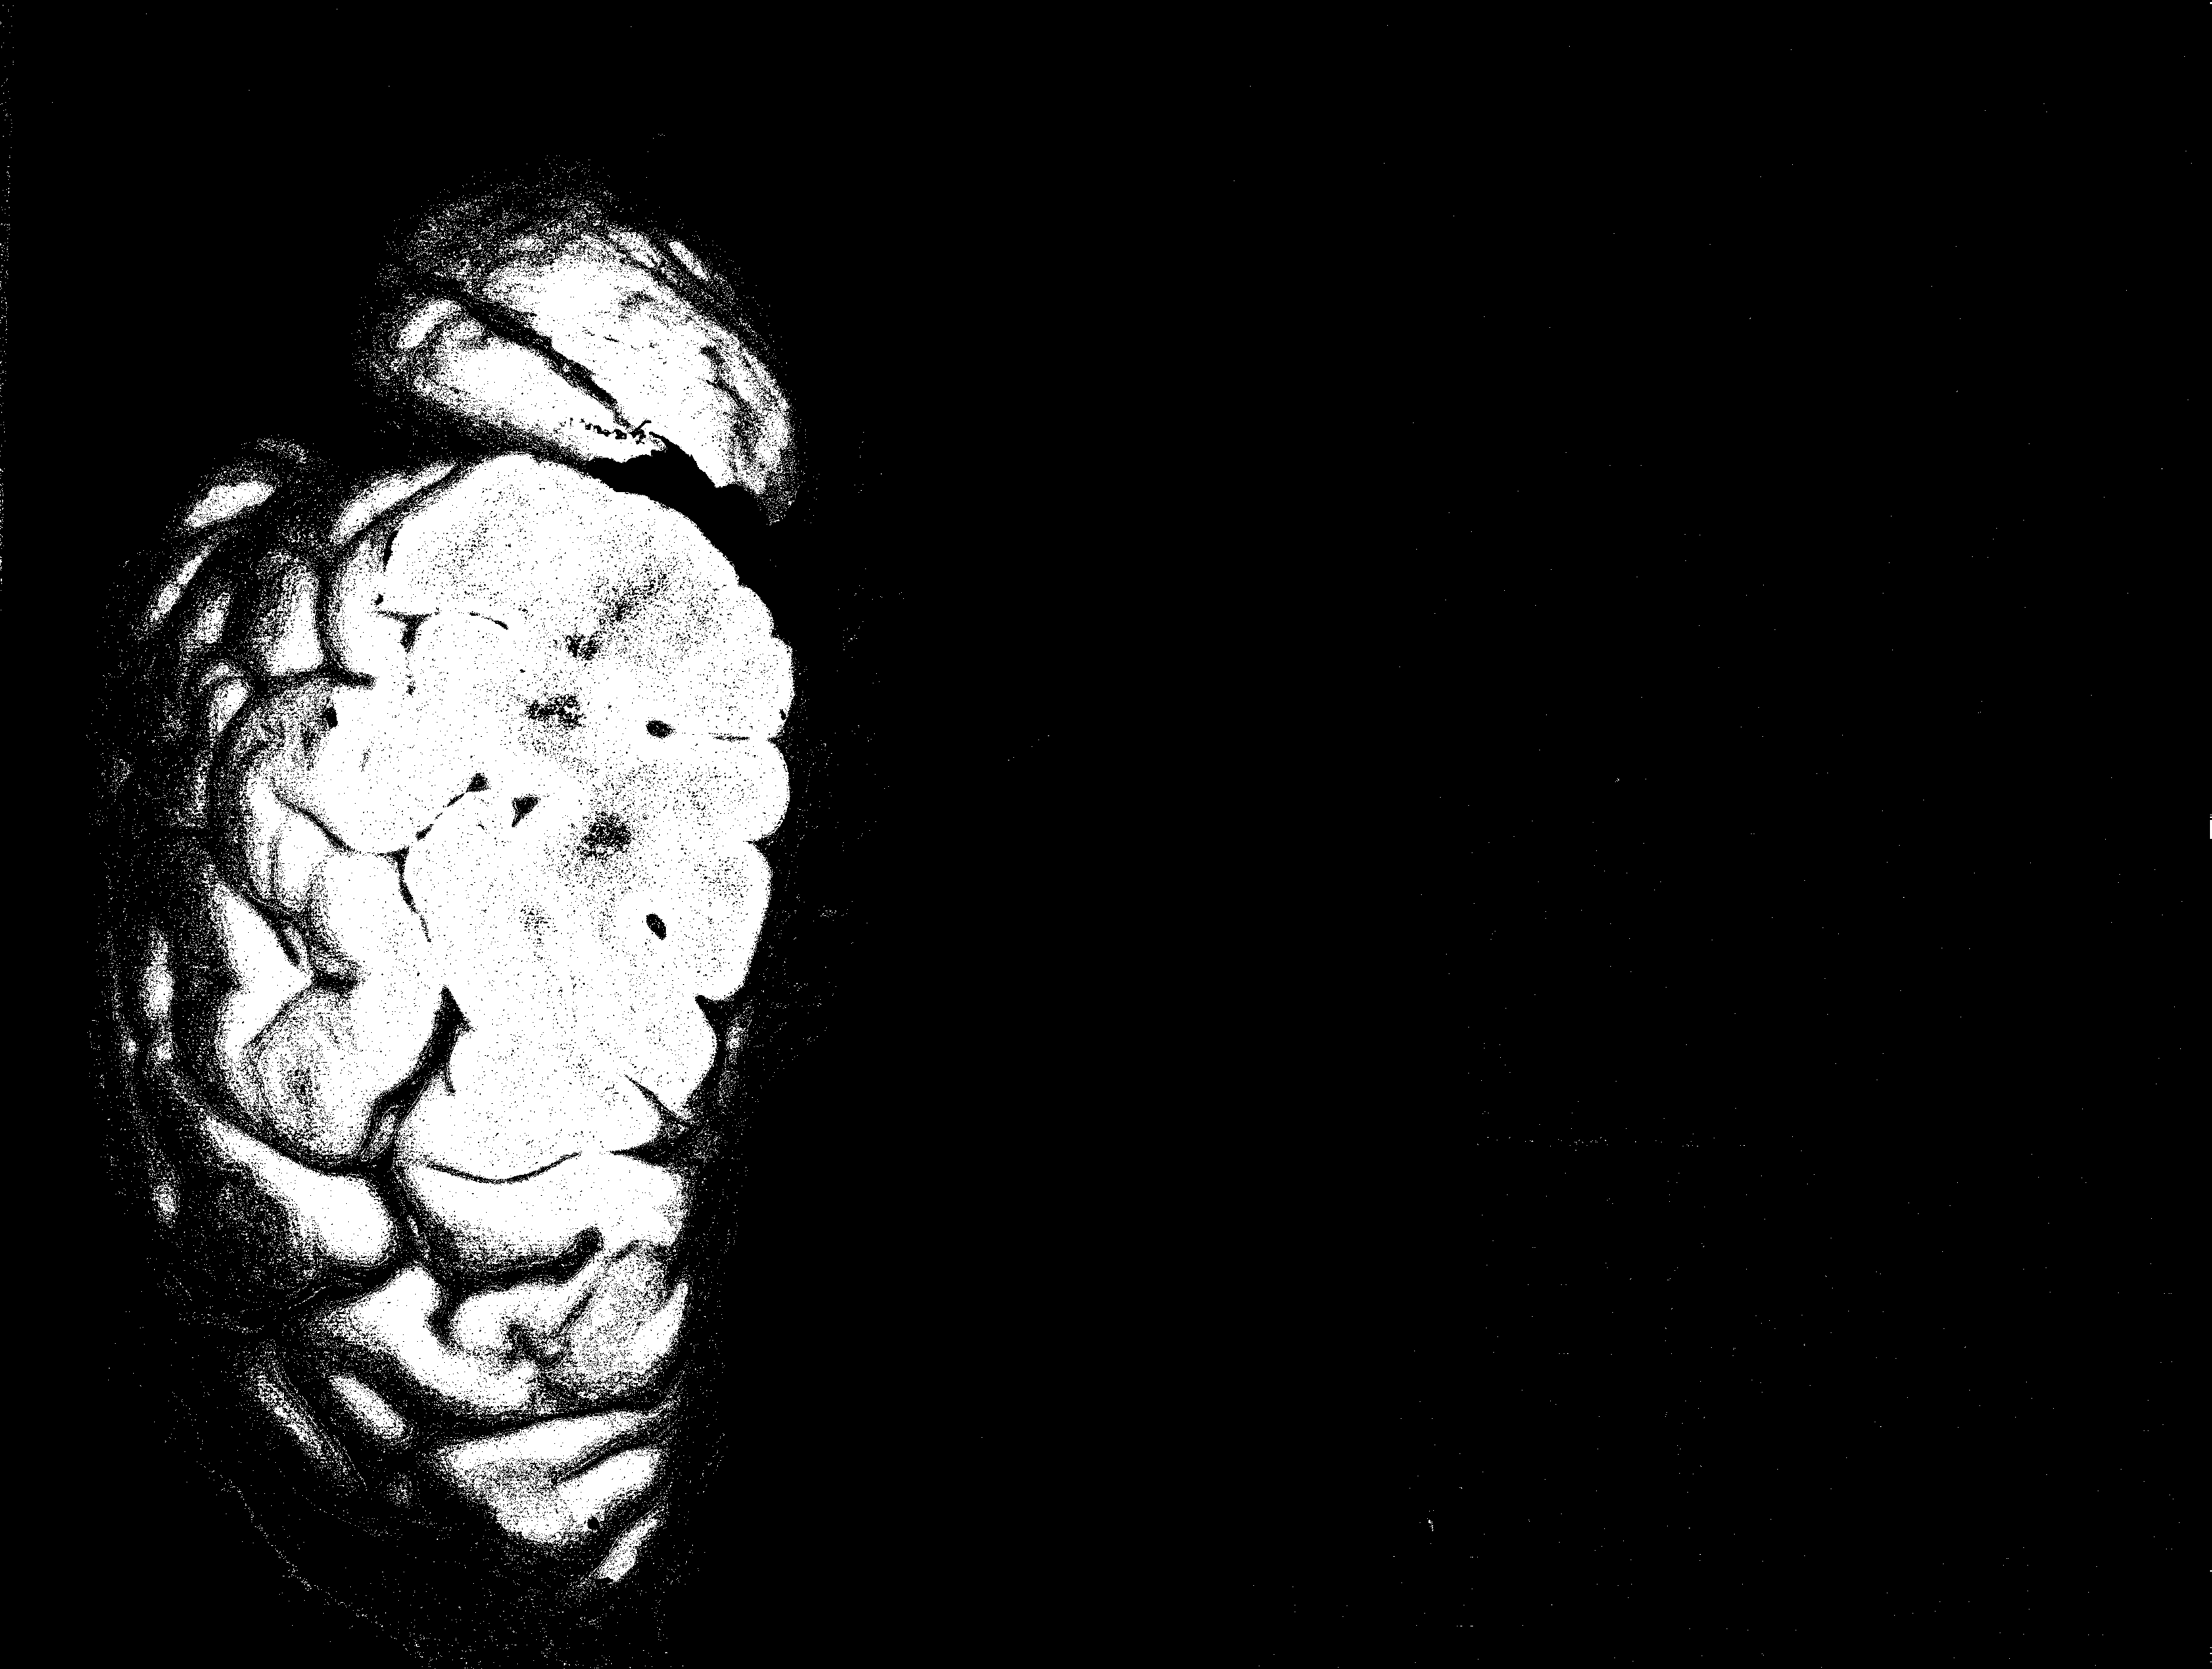
\includegraphics[width=0.7\linewidth]{graphics/predict200_svm_rbf} 
\caption{predicted image using svm with rbf kernel} 
\label{fig:predict200_svm_rbf} 
\end{figure}


\subsubsection{Local Features}

Despite adding the HSV color space, there is still no information
on the neighbourhood of a pixel. A first level approach to get information
on the neighbourhood of a pixel are statistical values like mean or
standard deviation. The statistical values are calculated on an $N\times N$
array around a pixel and assigned to the centered pixel. Listing \ref{calc_std}
shows how the standard deviation is calculated for an image. This
is done with the numpy and scipy modules. The \emph{generic\_filter}
function generates a window with the given size for every pixel and
calls the given function (e.g. numpy.std). The standard deviation
is an indication for the homogenity of the pixel's neighbourhood.

\begin{lstlisting}[basicstyle={\footnotesize\ttfamily},breaklines=true,caption={Calculate standard deviation},extendedchars=true,label={calc_std},language=Python,numbers=left,numberstyle={\tiny},showstringspaces=false,tabsize=2]
def calc_std(img,size,use_mean=False):     
	"""Calculate the local standard deviation for each pixel of an image.
    Arguments:
        img : rgb image
        size : size of the window of neighbouring pixels
        use_mean : boolean, if False the standard deviation of R,G and B value are calculated and return as a 3 dimensional array.
                    if True the standard deviation of the mean is returned.
    Return:
      array_like, 3d or 2d
    """
    if not use_mean:
        std = np.zeros(img.shape)
        for i in range(img.shape[2]):
            std[:,:,i] = filters.generic_filter(img[:,:,i],np.std,size)
    else:
        mean_img = np.mean(img,axis=2)
        std = filters.generic_filter(mean_img,np.std,size)
    return std
\end{lstlisting}


By using the local standard deviation as a feature some information
of the neighbourhood is used, but this can be improved with other
features.


\subsubsection{Image Segmentation}

A more complex feature can be achieved by performing watershed segmentation.
It is used on grayscale images and the pixel values are treated as
a elevation. The algorithm floods basins from markers, which were
set by the user. When two basins from different markers meet a watershed
is drawn. The markers can be set in an easy way by using thresholds.
While there are more complex ways using image processing methods,
the threshold approach is used to keep the feature generation simple


\subsection{Data Modeling}


\subsubsection{Support Vector Machines}

Support vector machines (SVMs) are one of the preferred classification
methods lately. They have a high accuracy, but their training time
is quite long. A model can easily be described by the found support
vectors.

SVMs can model nonlinear decision boundaries by using other kernels
instead of the linear kernel to increase the dimension of a vector.
A kernel defines the used scalar product. The most popular kernels
are the following:

\begin{itemize} 
\item linear:  $K(x,y) = \sum_{i=0}^n x_i\cdot y_i$ 
\item polynomial: $K(x,y) = (c+\sum_{i=0}^{n} x_i\cdot y_i)^d$	 	
\item rbf: $ \exp(-\frac{||x-y||^2}{2\sigma^2})$  
\end{itemize}  

\begin{figure}
\begin{tabular}{|l|r|r|r|}
\hline 	
Classifier 	& Accuracy & training time in s & test time in s \\  	
\hline 	
\hline 	
SVC (sklearn), rbf, 20k instances 	& 0.8752580408 	& 39.545465 	& 109.808209 	\\
\hline 	
\parbox[t]{6cm}{SVC (sklearn), rbf,\\ gamma=0.1, C=1, 20k instances} 	& 0.9579808675 	& 45.242423 	& 66.846724 \\  	
\hline 	
libSVM twister, 20k instances 	& 0.9592930497 	& 445.867 	& - \\  	
\hline 	
libSVM twister, 40k instances 	& 0.963317509 	& 934.912 	& - \\  	
\hline 	
libSVM twister, 100k instances 	& 0.9665214475 	& 3077.239 	& -\\ 	
\hline 
\end{tabular}  
\caption{SVMs from scikit-learn and Twister with rgb as features } 
\label{svm_table} 
\end{figure}

\begin{figure}
\begin{tabular}{|l|r|r|r|} 	
\hline 
Classifier & Accuracy & training time in s & test time in s \\  	
\hline 
GaussianNB & 0.9475908597 	& 0.042224 & 0.075098 \\  	
\hline
KNN & 0.9677196684 & 1.57 & 5.29\\
\hline
Decision Tree & 0.9569552165 	& 0.563767 	& 0.057934 	\\  	
\hline 
RandomForest  & 0.9637635858 	& 1.698716 	& 0.399092 \\  	
\hline  
\end{tabular}  
\caption{Different classifiers used with rgb features.} 
\label{different_classifiers_table} 
\end{figure}

More information on SVMs in general can be found at \cite{Han2011}.

Because support vector machines maximize the margin between the decision
boundary and the support vectors, they do not overfit as easily as
other classifiers like decision trees for example. However, solving
the quadratic problem can have a complexity between $O(n^{2})$ and
$O(n^{3})$ depending on the used algorithm and implementation. As
figure \ref{svm_table} shows training an svm takes much more time
to be trained than other classifiers. This is especially true if a
non linear kernel is used, e.g. rbf kernel. A linear svm is much faster
but this goes along with a drop in accuracy. To get both a feasible
training time and a good accuracy, a kernel approximation is used
together with a linear SVM. A kernel approximation is used before
training a SVM (see listing \ref{kernel approximation}). It adds
additional random features to the data. For the rbf kernel this is
done by a Monte Carlo approximation of its Fourier transform. More
information on random fourier features and random binning features
can be found at \cite{Rahimi}.
\begin{lstlisting}[caption={kernel approximation using scikti learn},label={kernel approximation},language=Python]
from sklearn.kernel_approximation import RBFSampler
rbf = RBFSampler(gamma=2) 
X_features = rbf.fit_transform(X_train) 
X_test_features = rbf.transform(X_test)
\end{lstlisting}


A second approach is the Nystroem method \cite{Williams01usingthe}
which can approximate every kernel and not only the rbf one. It uses
a subsample of the data set to approximate a kernel. As \cite{NIPS2012_4588}
shows the nystr�m method can achieve a better generalization in some
cases. For the brain analytics use case however this could not be
noted.

\begin{figure} 
\centering 
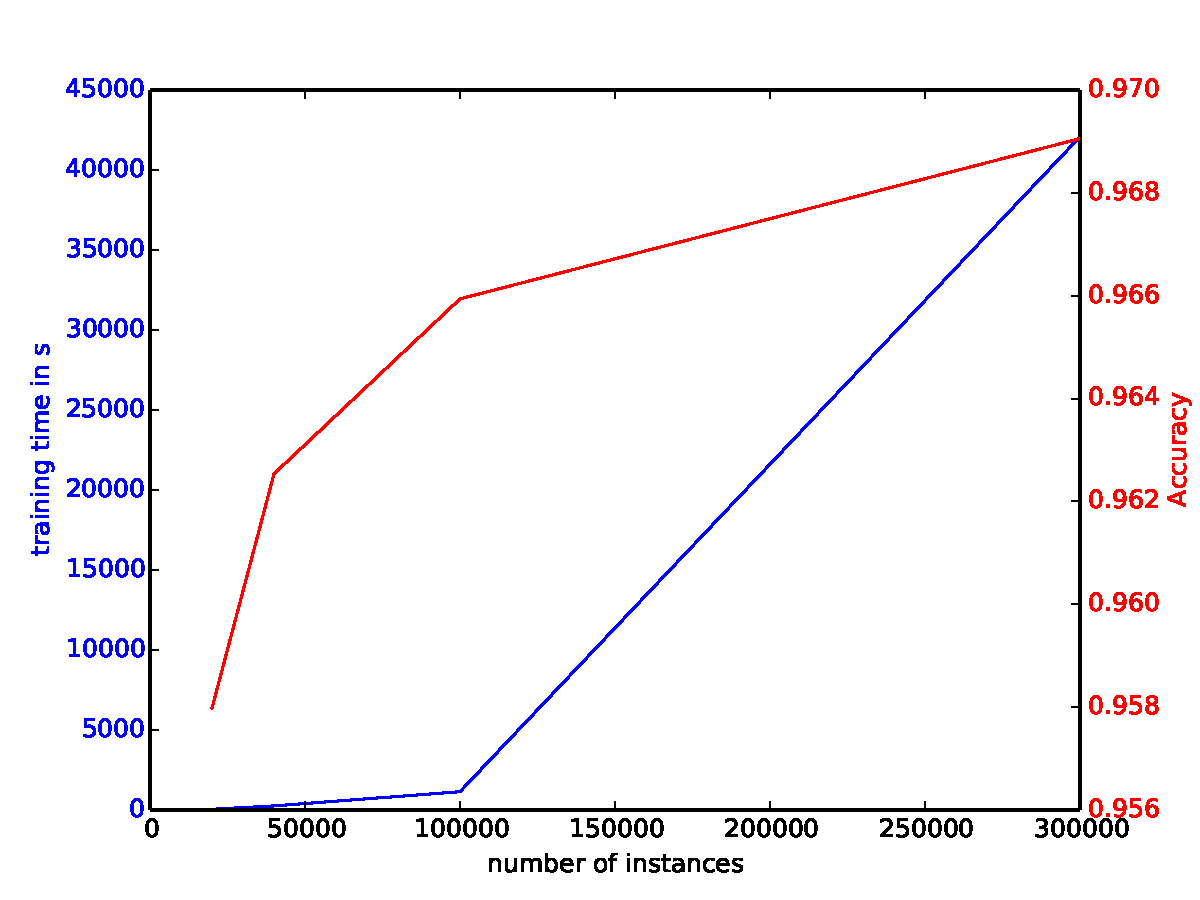
\includegraphics[width=0.8\linewidth]{graphics/sklearn_runtime} 
\caption{SVC training time with increasing sample} 
\label{fig:sklearn_runtime} 
\end{figure}


\subsubsection{Other Classifiers}

There are some other classifiers besides support vector machines.
While the focus is on SVMs and they were optimized the most, some
models with other classifiers were tested too. Naive Bayes is one
of them. Due to its simplicity it is quite fast. Unfortunatly the
accuracy score is not good since Naive Bayes assumes independency
of features which is obiously not the cause for RGB values of an image. 

While KNearestNeighbour considers feature dependencies and therefore
has a higher accuracy, it's training time is also higher than the
one of naive bayes. Apart from that figure \ref{different_classifiers_table}
shows that the prediction takes much longer since the distances to
all instances have to be calculated.

Decision trees have a better accuracy than naive bayes as well but
not as good as KNN. While their training time is larger than the one
of naive bayes, it is way faster than KNN. For the random forest classifier,
which uses ten randomized decision trees, the accuracy as well as
the training and testing time increase.


\subsubsection{Multiple Models}

With only one model for all the different cross section the prediction
is not very good for some cross sections. While it is not reasonable
to use the x and y coordinates of a pixel as features because the
brains position changes between the images, it is possible to use
the z axis as a feature. The z position of an image is contained in
its file name, since all the images are numbered. Naturally, for this
to work future cross sections have to be numbered in the same way.
The alternative to using the z position as a feature with one model
is to divide the brain in several layers and create a model for every
layer. 

This has several advantages in comparison to using one model. 
\begin{itemize}
\item simpler models 
\item less training data for each model
\item more specialized models
\end{itemize}

\subsubsection{Grid Search}

While scikit-learn already implements a function that performs grid
search on a given set of parameters and a classifier, this function
can not be used if kernel approximation is used as well. The parameters
that have to be optimized are the penalty parameter $C$ and kernel
coefficient $\gamma$. If kernel approximation is used, the linear
SVM does not expect an argument $\gamma$. Instead $\gamma$ is set
in the RBFSampler. Therefor the scikit-learn function can not be used
and a modified version was implemented. The new version generates
a new data set with the additional features and the current $\gamma$.
Thereafter a linear SVM is trained with the given $C$ and cross validated.
All results are saved in a list and returned. To speed up the grid
search, it is parallized with IPython using the LoadBalancedView.
Unlike the DirectView interface this one does not allow direct access
to the individual engines. Instead of that the IPython scheduler assigns
the tasks to the engines minimizing the idle time of the engines.


\subsection{Data Post Processing}

After the model is created an image can be predicted. During the preprocessing
the image is flattened and several features are added, so that every
row contains one pixel. Since the order of the pixel is contained,
the predicted labels can be reshaped to form a mask for the given
image. This gives a much better impression of the performance of the
model than the accuracy score because the data is not balanced. If
the mask of the image is given, the predicted mask and the original
mask can easily be compared by opening both masks or calling the \emph{compare\_to\_mask}
function. The latter calculates the accuracy, f-score and the confusion
matrix. Furthermore it also visualizes the confusion matrix as an
image. 


\subsection{Conclusion}\selectlanguage{british}%

